\begin{savequote}[75mm]
Add your quote here
\qauthor{Author of quote}
\end{savequote}

\chapter{Literature Review}
\label{literature}
\newthought{Lorem ipsum dolor sit amet}, consectetur adipiscing elit. Nunc neque massa, eleifend malesuada enim eu, efficitur imperdiet nulla. Aliquam augue est, lobortis eget scelerisque at, pretium vel lorem. Etiam faucibus nulla quam, nec tristique elit ullamcorper quis. Phasellus vel tincidunt nisl. Mauris at lacus sit amet mi auctor feugiat. Donec vel maximus erat. Suspendisse feugiat augue lacus, non egestas libero auctor sit amet. Nunc eros ante, posuere quis justo id, congue ultrices sapien.

\clearpage


\section{Machine Learning}


\subsection{Neural Networks}


\subsection{Deep Learning}



\subsection{Keras}




\section{Machine Translation}
\label{Machine Translation}


\subsection{Training Data}


\subsection{Techniques}

%\subsubsection{Rule-Based Machine Translation}


%\subsubsection{Statistical Machine Translation}


%\subsubsection{Transfer-Based Machine Translation}



%\subsubsection{Neural Machine Translation}


\subsection{Evaluation}


\clearpage

% Should this be under machine translation section?
\section{Corpus Augmentation}

\subsection{Back-Translation}
%Back-translation makes it possible to generate synthetic parallel data by pairing monolingual data with a back-translated version of the data.
Although monolingual data can be used to improve the performance of phrase-based \acrfull{SMT} using the language model, this is not the case for \acrshort{NMT}, where neural models are trained using parallel training data. Modern back-translation typically works by using \acrshort{NMT} to train a model that translates backwards from the target language to the source language. Once the model is trained, it is used to translate the monolingual data and create a synthetic parallel corpus. This can be visualised below in Figure \ref{fig:back_trans}.

\begin{figure}[ht!]
\centering
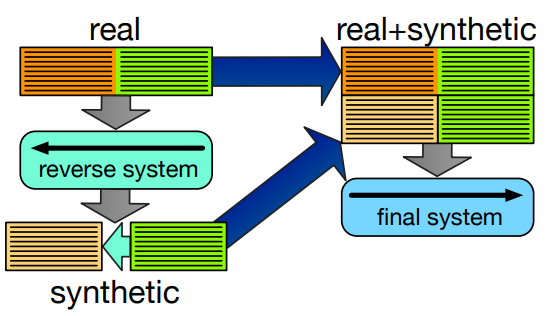
\includegraphics[width=0.45\textwidth]{media/literature/data_argumentation/da_back_trans.png}
\caption[Diagram of the back-translation synthetic parallel corpus]{Back-translation synthetic parallel corpus creation (\cite{hoang_iterative_2018})}
\label{fig:back_trans}
\end{figure}
%<<<<< There are various techniques, this is by \cite{hoang_iterative_2018} iterative back translation>>>>>
Research by \cite{sennrich_improving_2016} incorporates monolingual data into \acrshort{NMT} by studying the effect of using back-translation on monolingual data in order to improve translation models.  Without any alterations to the underlying architecture, their findings indicate that adding the synthetic data to the training corpus significantly improved translation quality by 3.4 BLEU score in both high-resource and low-resource training data sets.



% back-translation of monolingual target data into the source language,
% and treating this synthetic data as additional training data

% back translation is simple and easy to do as it doesn't require modification to MT training algorithms
% instead requires target to source system into order to generate additional synthetic parallel data
% from monolingual target data

% pairing monolingual training data with automatic back-translation,
% treat it as additional parallel training data
% Improvements on the low-resourced IWSLT 14 task Turkish > English (2.1 - 3.4 BLEU)
% state of the art results (in 2015)

% introduce back-translation technique for NMT
% shows the quality of the back-translation model, and therefore resulting pseudo-corpus
% has a positive effect on the quality of the subsequent source-to-target model

%\cite{graca_generalizing_2019} problems with sampling-based approaches + remedies
% current state of the art NMT models suffer from smearing issues (ott et al 2018)
% and are trained using label smoothing (pereyra et al, 2017)
% these result in low quality sampled sentences

% they investigate considering only high quality hypotheses by restricting search space of the model via:
% - ignoring words under a probability threshold during sampling
% - N-best list sampling

% Experiments show their restricted sampling techniques are comparable to or better than other generation methods
% by imitating human-generated data better

% translation quality is still not with consistent improvements over typical beam search strategy


%\cite{edunov_back_trans_2018} understanding back-translation at scale
% broadens understanding of back-translation
% investigates methods to generate synthetic source sentences
% scale to hundreds of millions of monolingual sentences and achieve new state of the art
% they found in low-resource settings, back-translation obtained by sampling or noised beam outputs
% are the most effective
% noise beam is sentences with various types of noise (deleting, replacing and swapping words)









\subsection{Sentence Segmentation}
\cite{zhang_corpus_2019} sentence segmentation:
\begin{itemize}
    \item Segmenting long sentences in a corpus using back-translation
    \item Generating pseudo-parallel sentence pairs
    \item Improves translation performance
\end{itemize}
% Segmenting long sentences in a corpus using back-translation
% and generating pseudo-parallel sentence pairs
% improves translation performance


\cite{fadaee_data_2017} more sentence segmentation:
\begin{itemize}
    \item Targets low-frequency words by generating new sentence pairs
    \item Containing new rare words in synthetically created contexts
    \item Improves translation quality up to 2.9 BLEU score over baseline
    \item Up to 3.2 BLEU score over back-translation
\end{itemize}
% Targets low-frequency words by generating new sentence pairs, containing new rare words
% in synthetically created contexts
% improves translation quality up to 2.9 BLEU over baseline
% and up to 3.2 over back-translation

\clearpage
\subsection{Easy Data Augmentation}
\acrfull{EDA} is a data augmentation technique which aims to improve \acrfull{NLP} text classification performance by creating augmented training data to artificially increase the size of the corpus. It is the corpus augmentation technique that uses a combination of word replacements, insertions, swaps, and deletions. Additional input parameters such as number of augmented sentences per original sentence, and the percentage of words from the original sentence to change allow for fine-tuning of the output relevant to the usage context. For each individual sentence in the training data, an augmented sentence is generated using an operation selected randomly from four different techniques:
\begin{itemize}
    \item \textbf{Synonym Replacement:} Select \textit{n} words at random and replace each one with a synonym
    \item \textbf{Random Insertion:} Insert the synonym of any word into any position. Repeat \textit{n} times
    \item \textbf{Random Swap:} Swap the position of any two words. Repeat \textit{n} times
    \item \textbf{Random Deletion:} Randomly delete each word with probability \textit{p}
\end{itemize}

\cite{wei_eda:_2019} found that \acrshort{EDA} increased model performance for both recurrent and convolutional neural networks and improvements are most significant when the data set was restricted to simulate a low-resource scenario. The additional training data generated and noise from the variety of swaps contribute towards reduced overfitting. In a text classification task, \acrshort{EDA} can achieve the same level of accuracy as the baseline performance of the entire training corpus despite only using only 50\% of the training corpus. Thus far, experiments of \acrshort{EDA} have focussed exclusively on its application to text classification. Therefore, it is unclear whether its benefits will be applicable in \acrshort{NMT} and is worth investigating further.

% say something about overfitting and how the context remains similar


% improves performance for convolutional and recurrent neural networks
% strong results for small data sets
% on average, only took 50% of the available training data to achieve the same accuracy as full data set

% contextual augmentation, noising, GAN or back-translation may work better, but:
% high cost of implementing relative to the expected performance gain
% EDA is a set of simple techniques that are generalisable to a range of NLP tasks

% added noise from random swaps can help prevent overfitting
% synonym is more likely to be relevant to the context and retain the original label of the sentence


%\begin{figure}[ht!]
%\centering
%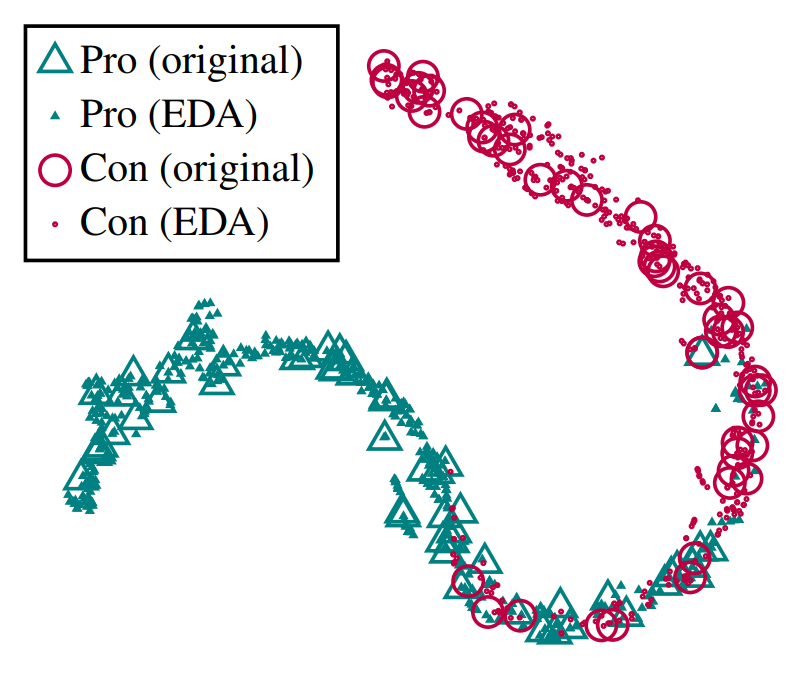
\includegraphics[width=0.45\textwidth]{media/literature/data_argumentation/eda_class.png}
%\caption[\acrshort{EDA} augmented data latent space visualisation]{EDA comparison of original and augmented sentences in a %latent space visualisation (\cite{wei_eda:_2019})
%}
%\label{fig:transfer}
%\end{figure}
\subsection{Contextual Data Augmentation}

Contextual data augmentation is a type of data augmentation where words are replaced at random using predictions from a language model, based on the context of the word within the sentence. As with other augmentation techniques, the primary aim is to reduce overfitting and improve generalisation of the models that train on the augmented data. 

Although capable of retaining contextual information, contextual data augmentation research is primarily focussed on text classification tasks rather than \acrshort{NMT}. Research by \cite{wu_conditional_2018} and \cite{kobayashi_contextual_2018} are good examples of this, where the augmented data is can be fairly similar to the original data making it significantly less beneficial for \acrshort{NMT} training despite remaining useful in \acrshort{NLP} classifiers. This is difficult to overcome due to limitations in the usage of vocabulary without repeating the augmentation process many times for each sentence while maintaining grammatically correct output.

\acrfull{SCDA} is a method of data augmentation proposed by \cite{zhu_soft_2019}, specifically designed for use in \acrshort{NMT} systems. The \acrshort{SCDA} uses a language model that is trained on the same training corpus as the \acrshort{NMT} model. As shown below in Figure \ref{fig:scda}, the key difference is that random words from the original sentences are replaced with a mix of contextually related words using a probability distribution vector.


\begin{figure}[ht!]
\centering
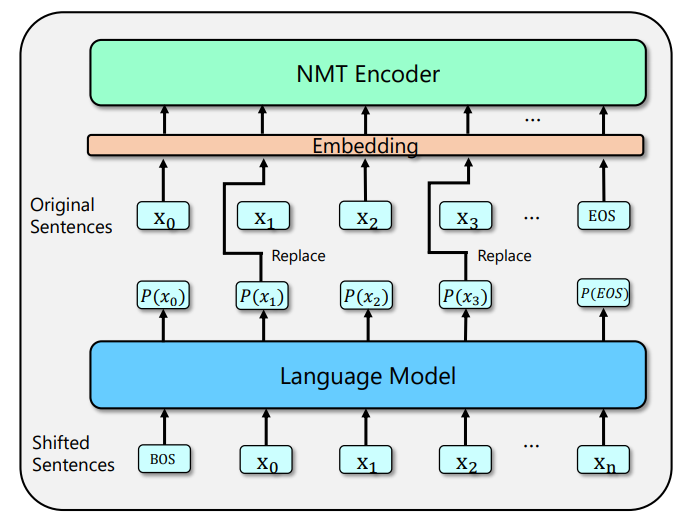
\includegraphics[width=0.6\textwidth]{media/literature/data_argumentation/da_scda.png}
\caption[Diagram of the \acrlong{SCDA} encoder architecture]{\acrlong{SCDA} encoder architecture (\cite{zhu_soft_2019})}
\label{fig:scda}
\end{figure}

Their findings demonstrate that the \acrshort{SCDA} method provides a consistent improvement of more than 1.0 BLEU score for transformer model \acrshort{NMT} in comparison to alternative approach baselines using a transformer model with both small and large data sets.

% Data augmentation is good in deep learning computer vision,
% it is still limited in natural language

% this paper presents a novel data augmentation method for NMT
% different from previous methods that drop swap or replace words with other words

% other methods often need to augment one sentence multiple times and replace
% a different subset of words in the original sentence with different candidate words in vocabulary
% which still cannot guarantee adequate variations of augmented sentences 

% they softly augment a random word in a sentence by its contextual mixture of multiple related words
% by replacing the one-hot representation of a word by a distribution over the vocabulary

% they use a distribution vector to replace a randomly chosen word from the original sentence

% results demonstrate superiority over baselines for small and large scale MT data sets
% consistently achieve more than 1.0 BLEU score improvement over strong Transformer base system for all tasks
% unlike other methods that may not work well in all tasks,
% theirs does, regardless of the data set




% The augmented data closely match the position of the original data,
\clearpage
\section{Low-Resource Machine Translation Approaches}
\label{LRNMT}


\subsection{Existing Scottish Gaelic Machine Translation}
%Existing research on Scottish Gaelic machine translation has focussed on using \acrshort{SMT}

Research by \cite{dowling_leveraging_2019} takes advantage of the increased data availability of a high-resource language (Irish Gaelic) and uses back-translation to create a parallel corpus with Scottish Gaelic, a closely related low-resource language pair. As shown in Figure \ref{fig:lang_pair}, the sentence structure of Irish Gaelic (GD) and Scottish Gaelic (GA) is very similar, making it an ideal choice for back-translation.

\begin{figure}[ht!]
\centering
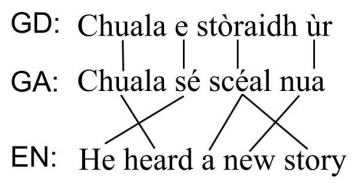
\includegraphics[width=0.4\textwidth]{media/literature/nmt_approaches/lr_gaelic.png}
\caption[Diagram of the similarities in a closely related language pair]{Similarities in a closely related language pair (\cite{dowling_leveraging_2019})}
\label{fig:lang_pair}
\end{figure}


The \acrshort{SMT} model saw improvements in performance over baseline when combining the synthetic training data with the original training data. The reason stated for not using \acrshort{NMT} in this research was due to the limited corpus size. As \acrshort{NMT} translation quality suffers significantly when models are trained with a low quantity of data, and as demonstrated in research by \cite{dowling_smt_2018}, a well tailored \acrshort{SMT} model achieves much better translation quality in comparison to an "out-of-the-box" \acrshort{NMT} model for Irish translation. Therefore, the research and implementation of low-resource machine translation approaches for Scottish Gaelic may contribute towards solving this problem.




\clearpage

\subsection{Transfer Learning}

As outlined by \cite{torrey_transfer_2009}, transfer learning uses the knowledge gained from a previous task in order to improve model performance in a related task. This concept is illustrated below in Figure \ref{fig:transfer}, where knowledge gained from the source domain Model A is used to help inform the target domain Model B.

\begin{figure}[ht!]
\centering
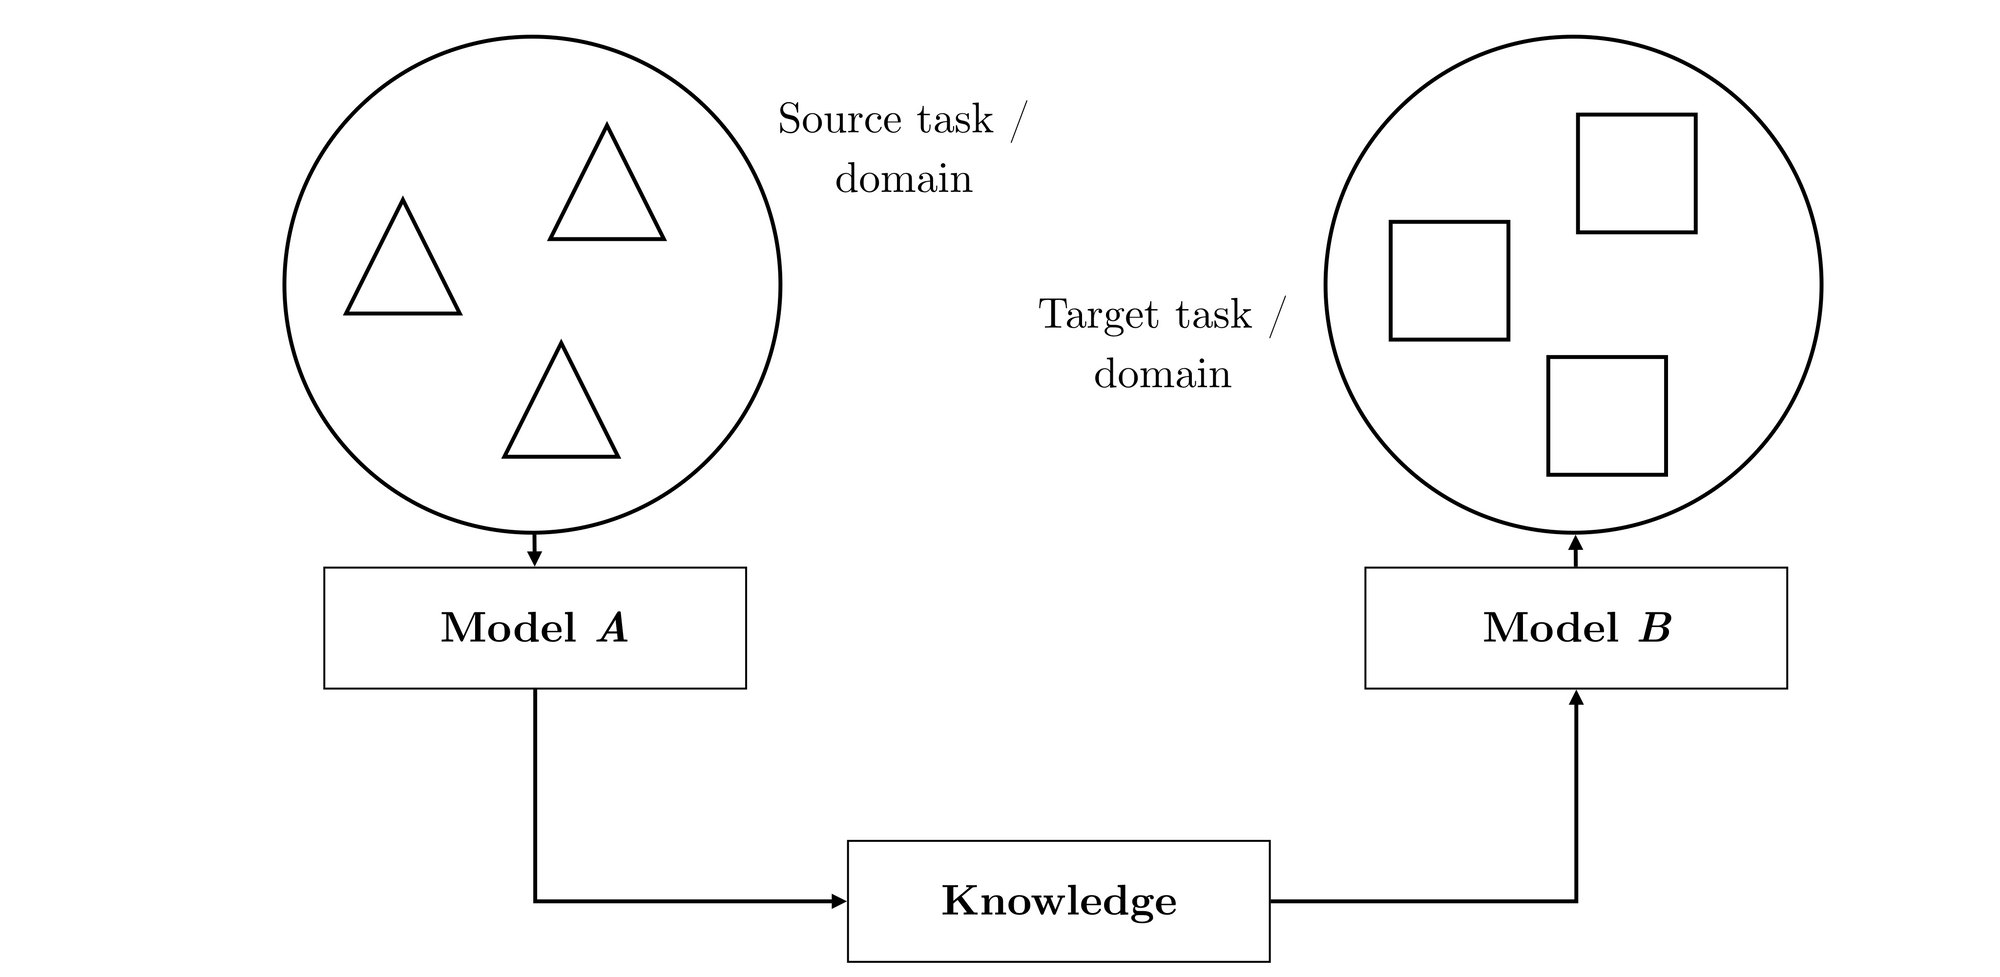
\includegraphics[width=0.85\textwidth]{media/literature/nmt_approaches/transfer.png}
\caption[Diagram of the transfer learning process]{The process of transfer learning (\cite{ruder_transfer_2019})}
\label{fig:transfer}
\end{figure}


In a neural machine translation context, this involves training a model with data from a high-resource language and then using that model to initialise the weights of the model the will be trained on the low-resource language.
This was demonstrated in research carried out by \cite{zoph_transfer_2016}, where transfer learning improved the performance of \acrshort{NMT} models for low-resource languages by an average of 5.6 \acrshort{BLEU} on four different language pairs. Results of the experiment also suggest that selecting a high-resource language closely related to the low-resource language can improve transfer learning models and therefore translation quality.

However, this contradicts more recent research by \cite{kocmi_trivial_2018} which looks at "trivial transfer learning". Existing transfer learning methods require a degree of language relatedness, whereas trivial transfer learning prioritises data quantity for the high-resource language. Their findings indicate that the relatedness of the language pair is of less importance than the quantity of data used in the initial high-resource language training. Despite being unable to pinpoint the exact reasoning behind the improvement in results, they state that "our observations indicate that the key factor is the size of the parent corpus rather than e.g. vocabulary overlaps".
It is worth noting that \cite{kocmi_trivial_2018} use a transformer neural network architecture instead of the recurrent neural network architecture used by \cite{zoph_transfer_2016}. Research by \cite{popel_training_2018} found that using the transformer model leads to better translation quality, likely contributing towards the contradictory results.


Hierarchical transfer learning seeks ensure the closeness of the related language pair, as identified in most transfer learning research, while simultaneously addressing the importance of the high-resource data quantity outlined in trivial transfer learning. \cite{luo_hierarchical_2019} achieve this by implementing three distinct stages of training:

\begin{itemize}
  \item Train the model using an unrelated high-resource language pair
  \item Initialise the next model and train on an intermediate language pair
  \item Initialise the final model and train using the low-resource language pair
\end{itemize}
% The first stage involves training using an unrelated high-resource language pair. Once the model has reached convergence, it is used to initialise the next model that will be trained on an intermediate language pair, closely related to the low-resource language. Upon convergence, the final model in the hierarchy is initialised and the low-resource language pair is trained.

Results indicate improvements of up to 0.58 \acrshort{BLEU} score in comparison to the aforementioned transfer learning methods that are limited to a parent-child architecture.


% Train the NMT model using the unrelated high-resource language pair
% Train using the similar intermediate language pair
% Train using the low-resource language pair


\subsection{Meta Learning}
% Seems like an extension of hierarchical transfer learning

% what is meta learning
Meta learning can be thought of as the machine learning process of "learning how to learn". Observing the performance of different approaches on a variety of tasks and then using this experience to influence the learning process of new tasks in order to considerably increase the rate of learning (\cite{vanschoren_meta-learning:_2018}).

% talk about model agnostic meta learning

\acrfull{MAML} is a meta learning algorithm proposed by \cite{finn_model-agnostic_2017}, where models are trained to adapt quickly. This leads to good a generalisation performance on a new task despite a low quantity of training data.
A diagram of the \acrshort{MAML} algorithm can be seen below in Figure \ref{fig:MAML}.

\begin{figure}[ht!]
\centering
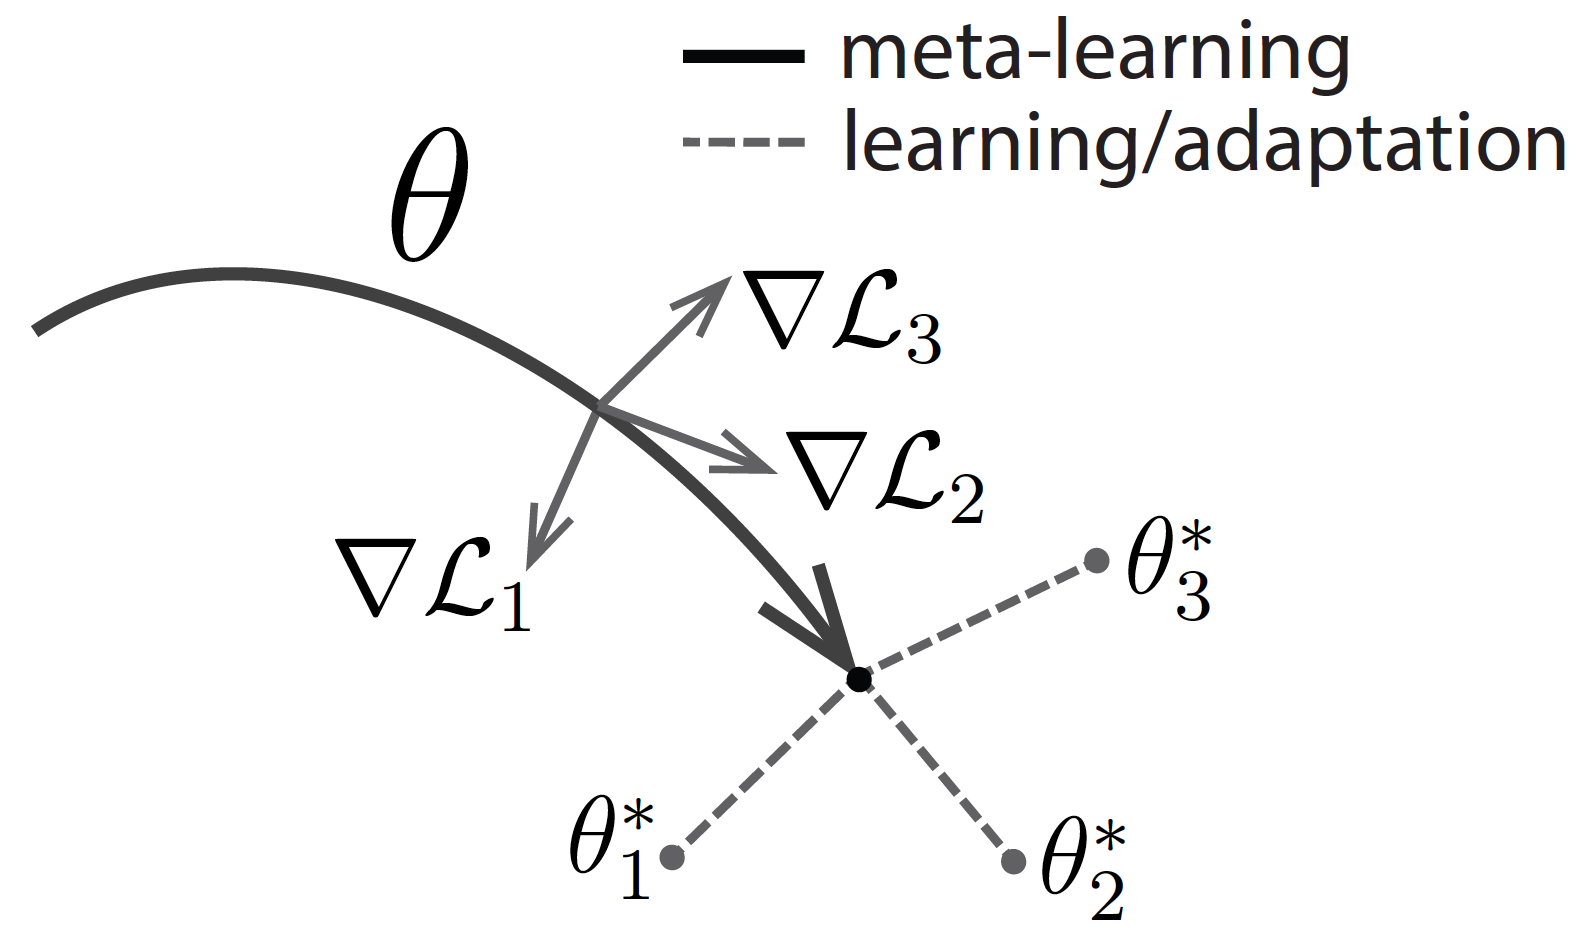
\includegraphics[width=0.45\textwidth]{media/literature/nmt_approaches/maml.png}
\caption[Diagram of a \gls{MAML} algorithm]{An illustration of the \Gls{MAML} algorithm (\cite{finn_model-agnostic_2017})}
\label{fig:MAML}
\end{figure}

Despite the primary focus of \acrshort{MAML} research relating to object recognition, it can be applied to a variety of machine learning problems with any number of training steps or training data because the algorithm still produces a weight initialisation, meaning no additional learning parameters are required.

% as shown below in Figure ~\ref{fig:MAML}.
% goal of meta learning is to train model on variety of tasks 
% so that it can solve new tasks w/ small number of training samples

% In MAML, parameters of the model are trained such that a small number of gradient steps
% with a small amount of training data from a new task will produce good generalisation performance on that task

% Essentially, trains the model to be easy to fine-tune 
%
% Leads to state-of-the-art-performance with few-shot image classification benchmarks
%

% say how this paper uses meta agnostic model for translation
Research by \cite{gu_meta-learning_2018} is the first of its kind to use \acrshort{MAML} for \acrshort{NMT}. In comparison to the transfer based approach by \cite{zoph_transfer_2016}, results showed further improvements with a BLEU score of 22.04, despite training data for the low-resource language limited to 16,000 words (around 600 parallel sentences). As the corpus size of the low-resource language decreases, transfer learning approaches suffer significantly more than meta learning, which proves the effectiveness of \acrshort{MAML} for low-resource languages. However, as the corpus size increases, the differences in BLEU score between the two approaches are much less significant.

\clearpage

\section{Conclusion}
